\section{Implementationsaspekte}

% *2. Implementierungsaspekt* Prozesse/Threads/Protothreads und ähnliches
% (10min - 15min)
%
% - Contiki Prozesse an Minimal-Beispiel zeigen und erklären
%   (compilieren, programmieren und ausführen)
% - Kommunikation zwischen Prozessen

\subsection{Theorie}
%-------------------------------------------------------------------------------
\begin{frame}{Theorie}{Anforderungen}
	\begin{description}[Programmierung]
	\item[Strom]
		Knoten sollen Jahre mit einer Batterie auskommen
		%\item[Reaktion]
			%relativ wenig Last, mehr reagieren
	\item[Speicher]
		nur wenige KB RAM
	\item[Programmierung]
		einfache Programmierung

		Netzwerkprotokolle sind kontrollfluss- und nicht zustandsorientiert
	\end{description}
\end{frame}

%-------------------------------------------------------------------------------
\begin{frame}{Theorie}{Systemarchitekturen}
	\begin{block}{ereignisgesteuert}
		\begin{proconlist}
		%\pro	Stromsparend (kein Polling)
		\pro	nur ein Stack \conclusion geringer Speicherbedarf
		%\contra	keine rechenintensiven Algorithmen
		\contra	Programmierung als Zustandsmaschine notwendig
		%\contra	nur neuestes Ereignis kann abgearbeitet werden
		%\contra	Ereignisbehandlung kann nicht unterbrochen werden
		\end{proconlist}
	\end{block}

	\begin{block}{threadorientiert}
		\begin{proconlist}
		%\pro	mehrere Behandlungen nebeneinander
		%\pro	größere Berechnungen möglich
		%\pro	Ereignisse können nach Wichtigkeit geordnet behandelt werden
		%\pro	Nebenläufigkeit
		\pro	intuitivere Programmierung, keine Zustandsmaschinen
			notwendig
		\contra	hohe Speicherreservierung je Thread
		%\contra	Außenwelt muss regelmäßig eigenständig abgefragt werden
			%\(\to\) hoher Stromverbrauch
		\end{proconlist}
	\end{block}
\end{frame}
%-------------------------------------------------------------------------------

\subsection{Protothreads}
%-------------------------------------------------------------------------------
\begin{frame}[fragile]{Protothreads}{Umsetzung der Makros (schematisch)}
	\begin{columns}
	\column{.40\linewidth}<1->
		\lstinputlisting[%
			keywords={do\_something\_else,do\_something,xyz},%
			title={Quellcode},%
			tabsize=4%
			]{impl/xmpl/protothread_before_precompiler.c}
	\column{.50\linewidth}<2->
		\lstinputlisting[%
			keywords={do\_something\_else,do\_something,xyz},%
			title={ausgewertete Defines},%
			tabsize=4]{impl/xmpl/protothread_after_precompiler.c}
	\end{columns}

	\uncover<3->{
	\begin{description}[CPU-Zuweisung]
	\item[CPU-Abgabe]
		return mit nächster Sprungmarke
	\item[CPU-Zuweisung]
		Funktionsaufruf mit Sprungmarke
		\begin{itemize}
		\item	lokale Variablen verlieren Werte bei Kontextwechsel
		\item	\alert{globale Variablen oder static nutzen}
		\end{itemize}
	\end{description}
	}
\end{frame}
%-------------------------------------------------------------------------------
\begin{frame}{Prozesse und Protothreads}
	\begin{description}[Protothread]
	\item[Prozess]
		ist einzelner Protothread
	\item[{Protothread}]
		\begin{itemize}
		\item	leichtgewichtiger Thread
		\item	\alert{kein} eigener Stack
		\item	kooperatives Multitasking
			\begin{description}[yield]
			\item[wait]	Protothread gibt Kontrolle ab, bis Event eintritt
			\item[yield]	Protothread gibt Kontrolle ab
			\end{description}
		\item	keine direkte Switchanweisung
		\end{itemize}
%		\begin{itemize}
%		\item	durch Macros realisiert
%		\item	\alert{kein} eigener Stack
%		\item	Variablen verlieren Werte bei Kontextwechsel
%			\begin{description}
%			\item[Lösung]	globale Variablen oder\newline static Variablen
%			\end{description}
%		\item	kooperatives Multitasking
%		\end{itemize}
	\end{description}
\end{frame}
%-------------------------------------------------------------------------------
%\begin{frame}{Prozesse als Protothreads}
%	\todo{frametitle}
%
%	\input{impl/img/protothread.tex}
%\end{frame}
%-------------------------------------------------------------------------------

\subsection{Interprozess-Kommunikation}
%-------------------------------------------------------------------------------
\begin{frame}{Kommunikation zwischen Prozessen}{Events und Polling}
	\begin{description}[Event]
	\item[Event]
		Signal an einen Prozess in die Event Queue einordnen
		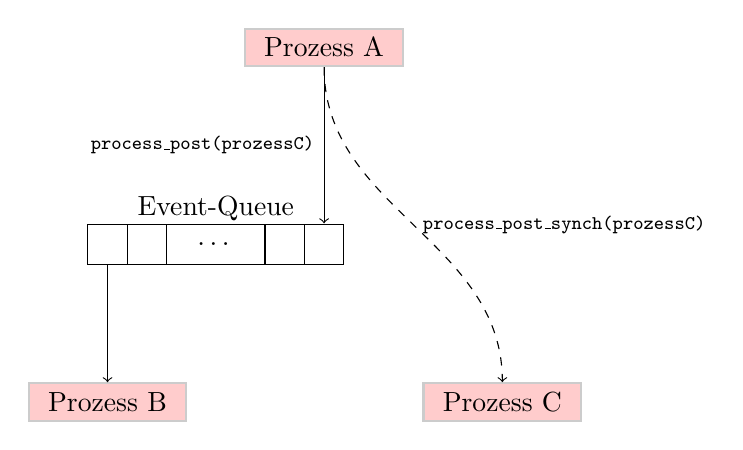
\begin{tikzpicture}
	\tikzstyle{aufruf}=[font=\ttfamily\scriptsize];
	\tikzstyle{funktion}=[draw,minimum width=2cm,fill=red!20,draw=black!20,thick];
	%\node (prozess) [funktion,below of=ph,below=1cm] {Prozess};


	\uncover<3->{
		\node [outer sep=0mm,inner sep=0mm] (eqout) at (0.25,0) {};
		\draw (0,0) -- (3.25,0) -- (3.25,.5) -- (0,.5) -- cycle;
		\draw (0.5,0) -- (0.5,0.5);
		\draw (1,0) -- (1,0.5);
		\node at(1.625,0.7) {Event-Queue};
		\node at (1.625,0.25) {\dots};
		\draw (2.25,0) -- (2.25,0.5);
		\draw (2.75,0) -- (2.75,0.5);
		\node [outer sep=0mm,inner sep=0mm] (eqin) at (3,.5) {};
	}
	\uncover<2->{\node (pa) [funktion,above of=eqin,above=1cm] {Prozess A};}
	\uncover<4->{\node (pb) [funktion,below of=eqout,below=.5cm] {Prozess B};}
	\uncover<5->{\node (pc) [funktion,right of=pb,right=3cm] {Prozess C};}

	\uncover<3->{\draw [->] (pa) -- node [aufruf,left] {process\_post(prozessC)} (eqin);}
	\uncover<4->{\draw [->] (eqout) -- (pb);}
	\uncover<5->{\draw [->] (pa) edge [in=90,out=270,dashed] node [aufruf,right] {process\_post\_synch(prozessC)} (pc);}
\end{tikzpicture}


	\uncover<6->{
	\item[Poll]
		\begin{itemize}
		\item	jeder Prozess besitzt Polling Flag
		\item	vor der Event Queue werden alle Polling Flags geprüft
		\item	bei gesetzten Polling Flag wird der Polling Handler ausgeführt
		\end{itemize}
		}
	\end{description}
\end{frame}
%-------------------------------------------------------------------------------
\begin{frame}{Kommunikation zwischen Prozessen}{Events und Polling im Einsatz}
	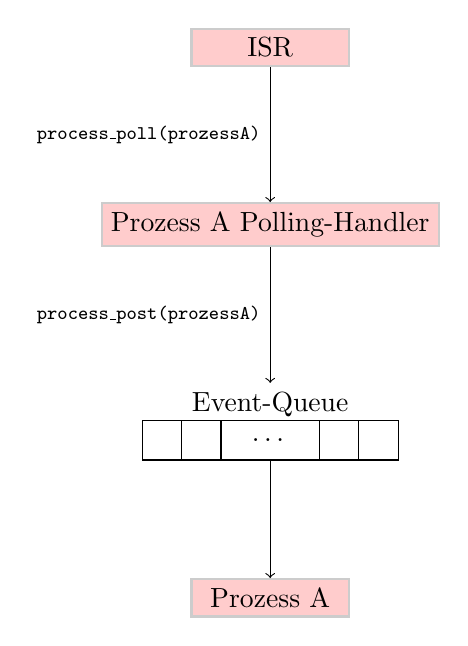
\begin{tikzpicture}
	\tikzstyle{aufruf}=[font=\ttfamily\scriptsize];
	\tikzstyle{funktion}=[draw,minimum width=2cm,fill=red!20,draw=black!20,thick];
	%\node (prozess) [funktion,below of=ph,below=1cm] {Prozess};


	\uncover<3->{
		\node [outer sep=0mm,inner sep=0mm] (eqout) at (1.625,0) {};
		\draw (0,0) -- (3.25,0) -- (3.25,.5) -- (0,.5) -- cycle;
		\draw (0.5,0) -- (0.5,0.5);
		\draw (1,0) -- (1,0.5);
		\node (eqin) at(1.625,0.7) {Event-Queue};
		\node at (1.625,0.25) {\dots};
		\draw (2.25,0) -- (2.25,0.5);
		\draw (2.75,0) -- (2.75,0.5);
	}
	\uncover<4->{\node (pa) [funktion,below of=eqout,below=.5cm] {Prozess A};}
	\uncover<2->{\node (ph) [funktion,above of=eqin,above=1cm] {Prozess A Polling-Handler};}
	\uncover<1->{\node (isr) [funktion,above of=ph,above=1cm] {ISR};}

	\uncover<2->{\draw [->] (isr) -- node [aufruf,left] {process\_poll(prozessA)} (ph);}
	\uncover<3->{\draw [->] (ph) -- node [aufruf,left] {process\_post(prozessA)} (eqin);}
	\uncover<4->{\draw [->] (eqout) -- (pa);}
\end{tikzpicture}

	%Literatur \url{http://www.sics.se/contiki/wiki/index.php/Processes}
\end{frame}
%-------------------------------------------------------------------------------
\begin{frame}{Kommunikation zwischen Prozessen}{Semaphore und Protosockets}
	\begin{description}[Protosockets]
	\item[Semaphore]
		zur Synchronisation der Protothreads
		\begin{itemize}
		\item	PT\_SEM\_INIT(s, c)
		\item	PT\_SEM\_WAIT(pt, c)
		\item	PT\_SEM\_SIGNAL(pt, c)
		\end{itemize}
	\item[Protosockets]
		Zugriff auf das uIP-Interface, analog zu BSD-Sockets
		\begin{itemize}
		\item	PSOCK\_INIT(\dots)
		\item	PSOCK\_SEND\_STR(\dots)
		\item	PSOCK\_READBUF(\dots)
		\item	\dots
		\end{itemize}
	\end{description}
\end{frame}
%-------------------------------------------------------------------------------

%-------------------------------------------------------------------------------
\subsection{Beispielprojekt}
%-------------------------------------------------------------------------------
%-------------------------------------------------------------------------------
\begin{frame}{Beispielprojekt}
	\begin{block}{Repository}
		\begin{itemize}
		\item	klonen\newline
			\texttt{git clone https://github.com/contiki-os/contiki}
		\item	anpassen
			\begin{itemize}
			\item	\texttt{contiki/cpu/avr/Makefile.avr}
				\begin{itemize}
				\item	\texttt{avrdude}
					\(\quad\to\quad\)
					\texttt{sudo avrdude}
				\end{itemize}
			\item	\texttt{platform/avr-atmegarfa1/Makefile.avr-atmegarfa1}
				\begin{itemize}
				\item	\texttt{AVRDUDE\_PROGRAMMER=jtag2}
					\(\quad\to\quad\)
					\texttt{dragon\_jtag}
				\item	\texttt{AVRDUDE\_PORT=usb:00B000000D79}
					\(\quad\to\quad\)
					\texttt{usb}
				\end{itemize}
			\end{itemize}
		\end{itemize}
	\end{block}
	\begin{block}{Projekt}
		\begin{itemize}
		\item	Projektverzeichnis erstellen\newline
			\texttt{mkdir -p project/hellosworld}
		\item	Bibliotheken des Sensorterminalboards kopieren\newline
			\texttt{config.h}, \quad
			\texttt{usb.c}, \quad
			\texttt{usb.h}, \quad
			\texttt{io\_access.c}, \quad
			\texttt{io\_access.h} \quad und \quad
			\texttt{io\_access\_ext.h} \quad
		\end{itemize}
	\end{block}
\end{frame}
%-------------------------------------------------------------------------------

%-------------------------------------------------------------------------------
\begin{frame}{Beispielprojekt}{hellosworld.c}
	\lstinputlisting[title={hellosworld.c},keywords={PROCESS,AUTOSTART\_PROCESSES,PROCESS\_THREAD,PROCESS\_BEGIN,PROCESS\_END}]{impl/xmpl/1st/hellosworld.c}
\end{frame}
%-------------------------------------------------------------------------------

%-------------------------------------------------------------------------------
\begin{frame}{Beispielprojekt}{Makefile}
	\begin{columns}
	\column{.55\linewidth}
		\lstinputlisting[title={Makefile}]{impl/xmpl/1st/Makefile}
	\column{.4\linewidth}
		\begin{block}{Verzeichnisbaum}
		\scriptsize
		\dirtree{%
			.1 contiki.
			.2 project.
			.3 hellosworld.
			.4 config.c.
			.4 hellosworld.c.
			.4 io\_access.c.
			.4 io\_access.h.
			.4 io\_access\_ext.h.
			.4 usb.c.
			.4 usb.h.
			.4 Makefile.
			.2 Makefile.include.
		}
		\end{block}
	\end{columns}
	\begin{itemize}
	\item	\texttt{make program}
	\end{itemize}
\end{frame}
%-------------------------------------------------------------------------------

